\documentclass[11pt]{article}

\usepackage[top=1.25in, bottom=1in, left=.8in, right=.8in]{geometry}

\usepackage{amsmath,amssymb,amsthm}
\usepackage{graphicx}


\newcommand{\pmu}{\, \partial_\mu }


%%%%%%%%%%%%%%%%%%%%%%%%%%%%%%%%%%%%%%%%%%%%%%
\begin{document}


\begin{figure}[t]
\centering
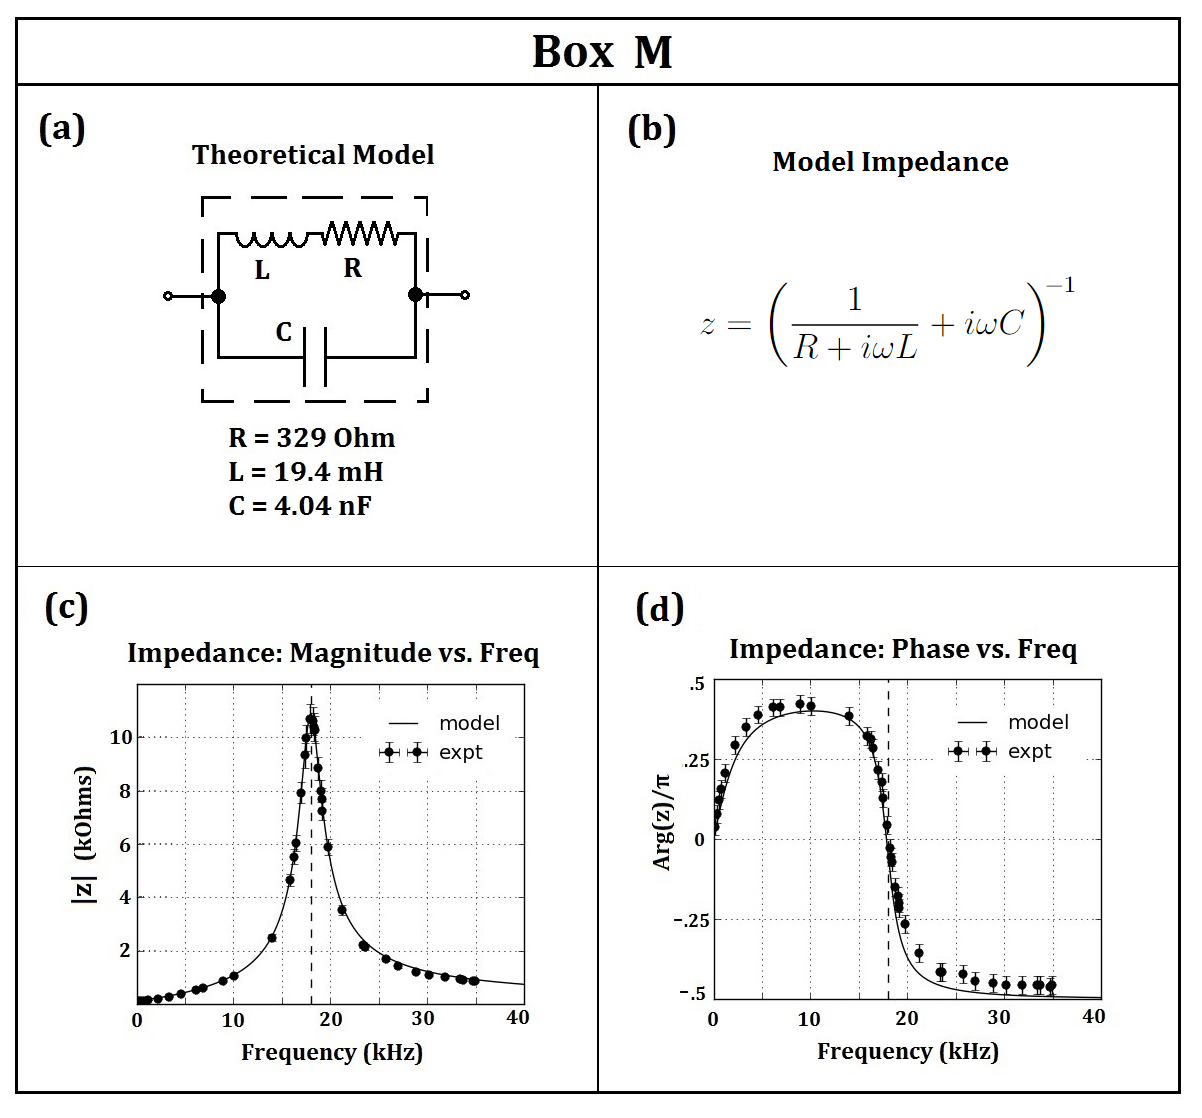
\includegraphics[scale=.5]{boxM.png}
\caption{Impedance versus frequency for Box M. A model for the unknown circuit is shown in \mbox{panel (a)}. The theoretical impedance associated with the model is given by the equation in panel (b). Panels (c,d) show the magnitude and phase of $z(f)$ for the experimental data (circles) and theoretical model (solid). Experimental data were obtained using the test circuit depicted in Figure 2. Error bars on the experimental data represent estimated uncertainties $\sigma_{|z|}=5\%$, $\sigma_{\phi}=5^{o}$, $\sigma_f = 100$Hz. Note that some error bars are small enough to be obscured by the symbols. Vertical dashed lines represent the model's nominal resonant frequency $f_0=17.986$kHz. The theoretical impedance of the model fits the data with reduced fit parameters $\chi^2_{|z|} = 9.34$ and $\chi^2_{\phi}=3.36$. It can also be shown that the fit is disrupted by parameter changes on the order of $5\%$. We conclude that this model approximates the unknown circuit in Box M to an overall accuracy of about $10\%$ in the 0-40kHz range, with a better fit near resonance and a poor fit near DC. A frequency-dependent model would be necessary to obtain a better fit over the entire range.}
\end{figure}



\clearpage

\begin{figure}[t]
\centering
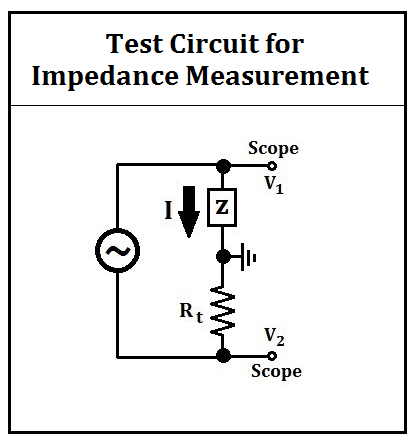
\includegraphics[scale=.6]{testcircuit.png}
\caption{Test circuit used to measure impedance of the unknown circuit element labelled $z$.}
\end{figure}































\end{document}
